\documentclass[10pt,a4paper,french]{beamer}
\usepackage{mmap}
\usepackage[utf8]{luainputenc}
\usepackage{polyglossia}
\usepackage{siunitx}
\setmainlanguage{french}
\usepackage{graphicx}
\usepackage{fontspec}
\usepackage{amsmath}
\usetheme{Darmstadt}
\usepackage{xcolor,colortbl}
\usepackage{subfig}
\definecolor{Orange}{HTML}{FFDD00}
\definecolor{Orange2}{HTML}{FFC000}
\definecolor{Green}{HTML}{8FB73E}
\definecolor{Green2}{HTML}{4EA700}
\definecolor{Red}{HTML}{EF4123}
\definecolor{Red2}{HTML}{EF2300}
%\usefonttheme[onlylarge]{structuresmallcapsserif}
%\usefonttheme[onlysmall]{structurebold}
\usepackage{etoolbox}
\useinnertheme{circles}
\newenvironment<>{vert}[1]{%
	\setbeamercolor{block title}{fg=black,bg=Green2}%
	\setbeamercolor{block body}{fg=black, bg=Green}%
	\begin{block}#2{#1}}{\end{block}}
\newenvironment<>{rouge}[1]{%
	\setbeamercolor{block title}{fg=black,bg=Red2}%
	\setbeamercolor{block body}{fg=black, bg=Red}%
	\begin{block}#2{#1}}{\end{block}}

%\setbeamercolor{block title}{use=structure,fg=structure.fg,bg=structure.fg!20!bg}
%\setbeamercolor{block body}{parent=normal text,use=block title,bg=block title.bg!50!bg}

%\setbeamercolor{block title example}{use=example text,fg=example text.fg,bg=example text.fg!20!bg}
%\setbeamercolor{block body example}{parent=normal text,use=block title example,bg=block title example.bg!50!bg}

\addtobeamertemplate{proof begin}{%
	\setbeamercolor{block title}{fg=black,bg=red!50!white}
	\setbeamercolor{block body}{fg=red, bg=red!30!white}
}{}

\mode<presentation>
\title{Caractérisation de détecteurs à plaques résistives de verres de basse résistivité en vue de la mise à niveau de CMS} 
\author{Lagarde François}
\date{20 Octobre 2017}
\institute{Institut de Physique Nucléaire de Lyon}

% logo of my university
\titlegraphic{%
	\includegraphics[width=2.5cm]{logo}\hspace*{4.75cm}~%
	\includegraphics[width=2cm]{logo2}
}

\begin{document}
	%titre
	\begin{frame}
		\titlepage
	\end{frame}
	%sommaire
	\begin{frame}
		\frametitle{Sommaire}
		\tableofcontents[pausesections]
	\end{frame}

	\section{Introduction}
	\subsection{Structure de la matière}
	\begin{frame}
		\begin{columns}
			\column{.6\textwidth}
			\includegraphics[height=0.7\textheight]{structure.jpg}
			\column{.4\textwidth}
			\end{columns}
	\end{frame}
	\subsection{Les particules élémentaires}
	\begin{frame}
	\begin{columns}
		\column{.6\textwidth}
		\includegraphics[height=0.7\textheight]{bestiaire.png}
		\column{.45\textwidth}
		\begin{block}{\centering Fermions (Spin demi-entier)}
			\setlength\abovedisplayskip{0pt}
			\begin{itemize}
				\item 6 quarks (anti-quarks)
				\item 6 leptons (anti-leptons)
			\end{itemize}
		\end{block}
		\begin{block}{\centering Bosons (Spin entier)}
			\setlength\abovedisplayskip{0pt}
			%\hspace*{.1\linewidth}\begin{minipage}{.8\linewidth}
			%\begin{block}{Médiateurs des interactions}
				\begin{itemize}
					\item 8 gluons (force forte)
					\item $\gamma$ (électromagnétisme)
					\item $Z^{0}$ $W^{\pm}$ (force électrofaible)
				%\end{itemize}
			%\end{block}
			%\end{minipage}
			%\begin{itemize}
				\item Boson de Higgs
			\end{itemize}
		\end{block}
	\end{columns}
	\end{frame}
	\subsection{Le Modèle Standard}
	\begin{frame}
	    \begin{block}{\centering Le modèle standard}
	    	\begin{itemize}
	    		\item Théorie non-abélienne
	    		\item Théorie perturbative
	    		\item Théorie quantique des champs (relativiste et quantique)
	    		\item l'ensemble des informations de la théorie est contenue dans un Lagrangien $\mathcal{L_{MS}}$
	    	\end{itemize}
	    \end{block}
		\begin{block}{\centering Lagrangien du Modèle Standard}
			\begin{equation}
			\only<1>{\mathcal{L_{MS}}=\textcolor{red}{\mathcal{L}_{\mathrm{Yang-Mills}}}+\mathcal{L}_{\mathrm{Dirac}}+\mathcal{L}_{\mathrm{Higgs}}+\mathcal{L}_{\mathrm{Yukawa}}}
			\only<2>{\mathcal{L_{MS}}=\mathcal{L}_{\mathrm{Yang-Mills}}+\textcolor{red}{\mathcal{L}_{\mathrm{Dirac}}}+\mathcal{L}_{\mathrm{Higgs}}+\mathcal{L}_{\mathrm{Yukawa}}}
			\only<3>{\mathcal{L_{MS}}=\mathcal{L}_{\mathrm{Yang-Mills}}+\mathcal{L}_{\mathrm{Dirac}}+\textcolor{red}{\mathcal{L}_{\mathrm{Higgs}}}+\mathcal{L}_{\mathrm{Yukawa}}}
			\only<4>{\mathcal{L_{MS}}=\mathcal{L}_{\mathrm{Yang-Mills}}+\mathcal{L}_{\mathrm{Dirac}}+\mathcal{L}_{\mathrm{Higgs}}+\textcolor{red}{\mathcal{L}_{\mathrm{Yukawa}}}}
			\end{equation}
			\begin{itemize}
				\item {\only<1>{\color{red}}$\mathcal{L}_{\mathrm{Yang-Mills}}$ Partie cinétique des champs de jauges.}

				\item {\only<2>{\color{red}}$\mathcal{L}_{\mathrm{Dirac}}$ Interactions entre fermions et bosons de jauges.}

				\item {\only<3>{\color{red}}$\mathcal{L}_{\mathrm{Higgs}}$ Donne la masse aux bosons $Z^{0}$,$Z^{\pm}$.}

				\item {\only<4>{\color{red}}$\mathcal{L}_{\mathrm{Yukawa}}$ Interactions entre le boson de Higgs et les fermions (donne une partie de la masse des fermions).}
			\end{itemize}
		\end{block}
	\end{frame}
	\subsection{Succès et lacunes du Modèle Standard}
	\begin{frame}
	\begin{columns}
		\column{.5\textwidth}
		\begin{vert}{\centering Ses succès}
			\begin{itemize}
				\item Prédiction du courant neutre
				\item Théorie renormalisable
				\item Excellents accords avec les mesures expérimentales 
			\end{itemize}
			\vspace*{-0.5cm}
			\begin{figure}[ht!]
				\centering
				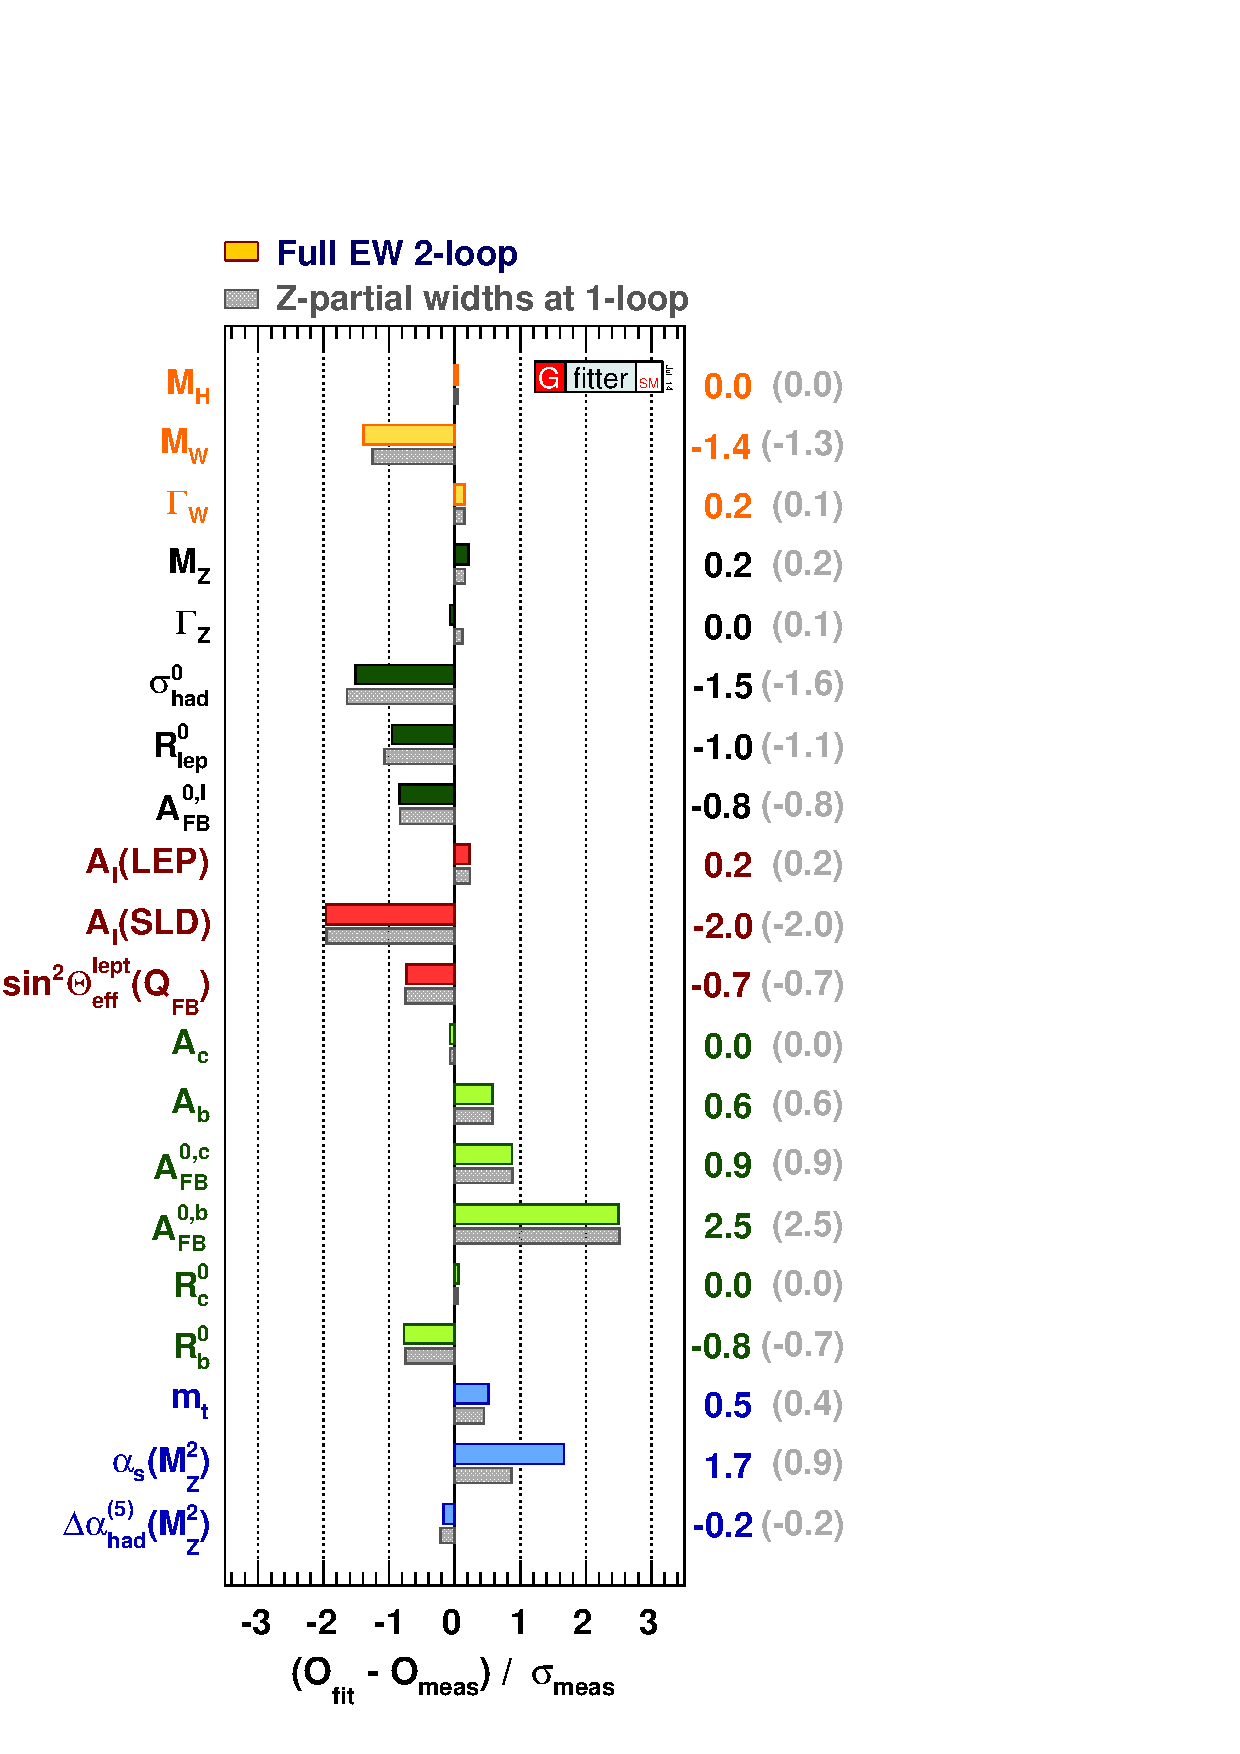
\includegraphics[width=0.60\textwidth]{mesure.png}
				%\caption{Comparaison des résultats d'ajustement avec les mesures directes de certains paramètres du Modèle Standard.}
			\end{figure}
		\end{vert}
		\column{.5\textwidth}
		\begin{rouge}{\centering Ses lacunes}
		\begin{itemize}
			\item Le nombre de familles
			\item Asymétrie baryon-antibaryons
			\item Gravitation non inclue
			\item Matière Noire et Énergie Noire 
			\includegraphics[width=0.50\textwidth]{darkmatter.png}
			\item Le nombre important de paramètres libres
			\item Neutrinos massifs
			\item non unification des couplages
			\item Naturalité
		\end{itemize}
		\end{rouge}
	\end{columns}
	\end{frame}
	\subsection{Au-delà du Modèle Standard}
	\begin{frame}
		\begin{block}{\centering Modèles au-delà du Modèle standard}
			Extension du Modèle Standard :
			\begin{itemize}
				\item \textit{Grand Unified Theories} : unifier les interactions sous une même symétrie.
				Basé sur un groupe $G\supset SU(3)\times SU(2) \times U(1)$
				\item Supersymétrie (SuSy) : supprimer le problème de la naturalité en associant à chaque fermions un  boson superpartenaire et réciproquement. 
				\begin{figure}
					\centering
					\includegraphics[width=0.60\textwidth]{SuSy.png}
				\end{figure}
				\item Modèle avec dimensions supplémentaires enroulées.
			\end{itemize}
		\end{block}
	\end{frame}
	\subsection{Le complexe d'accélération du CERN}	
	\begin{frame}
	    	\begin{columns}
	    		\column{.5\textwidth}
	    		\includegraphics[width=1.1\textwidth]{complexe.png}
	    		\column{.5\textwidth}
	    		\begin{block}{ Pour les collisions proton-proton}
	    			\begin{itemize}
	    				\item LINAC 2 ($\SI{50}{\mega\eV}$)
	    				\item BOOSTER ($\SI{1.4}{\giga\eV}$)
	    				\item {\only<2>{\color{red}}Synchrotron à protons (PS) ($\SI{25}{\giga\eV}$)}
	    				\item {\only<3>{\color{red}}SuperSynchrotron à protons (SPS) ($\SI{450}{\giga\eV}$)}
	    				\item Large Hadron Collider (LHC) ($\SI{7}{\tera\eV}$)
	    			\end{itemize}
	    		\end{block}
	    \end{columns}
		\only<2>{\begin{block}{\centering Ligne de faisceaux (East Area)}
			\begin{itemize}
				\item Particules : électrons, hadrons, muons...
				\item quantité de mouvement : \SIrange{1}{15}{\giga\eV}
				\item Intensité du faisceau : $\sim1-2\times 10^{6}$part/Spill
				\item Structure du Spill : 
				\begin{itemize}
					\item \SI{400}{\milli\second} 
					\item 1 Spill toute les \SI{33}{\second} (ou plus)
				\end{itemize}
			\end{itemize}
		\end{block}}
		\only<3>{\begin{block}{\centering Ligne de faisceaux (North Area)}
				\begin{itemize}
					\item Particules : électrons, hadrons, muons...
					\item quantité de mouvement : \SIrange{10}{400}{\giga\eV}
					\item Intensité du faisceau : $\sim1-2\times 10^{8}$part/Spill
					\item Structure du Spill : 
					\begin{itemize}
						\item \SIrange{4.8}{9.6}{\second} 
						\item 1 Spill toute les \SIrange{14}{48}{\second}
					\end{itemize}
				\end{itemize}
		\end{block}}
	\end{frame}
	\subsection{Le LHC}
	\begin{frame}
	\begin{columns}
		\column{.5\textwidth}
		\includegraphics[width=0.99\textwidth]{lhc-schematic.jpg}
		\column{.65\textwidth}
		\begin{block}{Le LHC}
			\begin{itemize}
				\item Collisions p-p, ion-ion, ion-proton
				\item \SI{27}{\kilo\meter} de circonférence
				\item 600 000 collisions par seconde
				\item $\sqrt{s}=\SI{14}{\tera\eV}$
				\item Luminosité instantanée $\sim\SI{e34}{\per\square\centi\meter\per\second}$
				\item \textit{pile-up} $\sim\num{40}$
			\end{itemize}
		\end{block}
	\end{columns}
	\begin{block}{\centering Quatre expériences principales}
			\begin{figure}
			\subfloat[ALICE]{\includegraphics[width=.2\linewidth]{alice.png}}
			\hfill
			\subfloat[ATLAS]{\includegraphics[width=.2\linewidth]{atlas.png}}
			\hfill
			\subfloat[LHC-b]{\includegraphics[width=.2\linewidth]{lhcb.png}}
			\hfill
			\subfloat[CMS]{\includegraphics[width=.2\linewidth]{cms.png}}
		\end{figure}
	\end{block}
	\end{frame}
    \subsection{Le HL-LHC}
    \begin{frame}
    \begin{columns}
    	\column{.6\textwidth}
   	\begin{block}{\centering Le HL-LHC (2023-2035)}
   	Augmenter la luminosité $\mathcal{L}(t)$ ($\times$ \SIrange{5}{7}{}):
   	\begin{equation}
   	N_{event}=\int \mathcal{L}(t)\sigma \mathrm dt
   	\end{equation}
   	\begin{itemize}
   		\item $\sigma$ est la section efficace du processus
   		\item $t$ la durée de prise de données
   		\item $\mathcal{L}$ la luminosité instantanée délivrée par le LHC.
   	\end{itemize}
     	\end{block}
   \column{.5\textwidth}
   \only<1>{\includegraphics[width=1\textwidth]{roadmap.png}}
   \only<2-3>{\includegraphics[width=1\textwidth]{man.jpg}}
   	\end{columns}
   \visible<3>
  	{
  		\begin{block}{}
  		{\color{red}Augmentation de la luminosité $\Rightarrow$ Augmentation du \textit{pile-up} ($\sim$ 140-200) et du flux de particules dans les détecteurs $\Rightarrow$ Mise à niveau de CMS.}
  		\end{block}
  	}
	\end{frame}
	\subsection{CMS}
	\begin{frame}
	\begin{block}{\centering CMS}
		\only<1>{\includegraphics[width=0.95\textwidth]{cms_empty.png}}
		\only<2>{\includegraphics[width=0.95\textwidth]{cms_tracker.png}}
		\only<3>{\includegraphics[width=0.95\textwidth]{cms_em.png}}
		\only<4>{\includegraphics[width=0.95\textwidth]{cms_ha.png}}
		\only<5>{\includegraphics[width=0.95\textwidth]{cms_ha.png}}
		\only<6>{\includegraphics[width=0.95\textwidth]{cms_spectro.png}}
	\end{block}
	\end{frame}
	\section{RPC}
	\section{Électrodes de verre de basse résistivité}
	\section{Électronique pour le timing}
	\section{Conclusion}
\end{document}
